\documentclass{article}
\usepackage[utf8]{inputenc}
\usepackage[russian]{babel}
\usepackage{enumitem}

\title{Design document}
\date{November 2024}

\begin{document}

\section{Введение}
Организация содержимого документа соответствует принятому стандарту оформления диздока.
Авторы: Береснев Вадим, Варакин Владислав, Громова Дарья, Демина Дарья, Мальцев Владислав, Попов Роман.

\section{Концепция}

\subsection{Введение}
Игра "Путешествие Лили" — это увлекательный платформер для детей и подростков, в котором игроки помогают любопытной лягушке Лили исследовать мир, собирая насекомых и избегая врагов на протяжении различных уровней, включая захватывающие битвы с боссами. Игрокам предстоит развивать ловкость и стратегическое мышление, чтобы преодолевать препятствия и открывать новые локации, узнавая интересные факты о фауне и экосистемах разных мест.

\subsection{Жанр и аудитория}
\begin{itemize}
    \item \textbf{Жанр:} платформер с элементами экшена и приключения
    \item \textbf{Возрастная группа:} 6+. Игра подходит для широкой аудитории.
    \item \textbf{Другие сведения о позиционировании игры:} образовательная и познавательная наклонность
\end{itemize}

\subsection{Основные особенности игры}
Попадая в новой мир, лягушка знакомится с другими лягушками, которые обитают в соответствующем биоме. Каждый мир представляет собой существующую климатическую зону, а местные лягушки, насекомые, птицы и змеи соответствуют действительно живущим в данных климатических зонах животным. При открытии нового мира игроку показывается справочная информация о лягушке, насекомых, птицах и змеях, которых игрок встретит в этом мире (название, внешний вид в реальном мире, ареал обитания, особенности, интересные факты). Таким образом, игра интересна не только процессом геймплея, но и познавательной стороной.

\subsection{Описание игры}
Игрок управляет лягушкой Лили, цель которой - увидеть мир, состоящий из 5 локаций. Для того чтобы попасть в другую локацию, необходимо договориться с животным, которое может перенести игрока (птица\крот и.т.д). Животное попросит трофей, получив который она будет готова перенести лягушку. На каждой локации будет 6 уровней, последний из которых – уникальная битва с боссом. На первых пяти уровнях игра представляет собой платформер, с препятствиями, врагами и насекомыми, которых лягушка может собирать. Для этого необходимо прицелится и выстрелить языком, точно попав по цели. Игроку необходимо успеть дойти до конца уровня за отведенное время. Уровень перезапускается если Лили получает урон или заканчивается время. За количество собранных насекомых, после каждого уровня игрок получит от одной до трех звезд. Перед уровнем с боссом будет возможность потратить накопленные звезды на различные улучшения (урон от удара языком, расходник защищающий от одного удара босса, и.т.д). Битва с боссом будет отличаться специальным условием победы, уникальным для каждого. После победы над боссом игрок будет получать трофей, необходимый для попадания на следующую локацию.


\subsection{Предпосылки создания}

\subsubsection{Общие тенденции рынка}

Рынок игр платформеров и адвенчур остается стабильным и востребованным, особенно в сегменте инди-игр. Платформеры, такие как \textit{Hollow Knight}, \textit{Celeste} и \textit{Ori and the Blind Forest}, демонстрируют устойчивый интерес аудитории благодаря сочетанию увлекательного геймплея, интересных персонажей и визуально привлекательных миров. Уникальная механика игры, где игрок управляет лягушкой с использованием языка для взаимодействия с окружением и борьбы, добавляет свежесть в жанр. Элементы сбора ресурсов и система звезд обеспечивают высокую реиграбельность, что важно для привлечения игроков к повторному прохождению уровней. 

Кроме того, комбинация платформера и адвенчуры, наряду с яркой, дружелюбной атмосферой, делает игру привлекательной для широкой аудитории, включая детей, подростков и казуальных геймеров, что соответствует современным трендам.

\subsubsection{Вопросы лицензирования}

Нет лицензии (пока что)

\subsection{Технические требования}
\begin{center}
\begin{tabular}{ c | c | c }
 & Минимальные технические & Рекомендуемые технические \\ 
 & требования & требования \\ [2ex]
 Операционная система & Windows 10 & Windows 10, 11 \\ [2ex] 
 Процессор & AMD Ryzen 3 1200 & AMD Ryzen 3 4100 \\  
 & Intel i3-8100 & Intel i3-12100 \\ [2ex]
 ОЗУ & 4 GB & 8 GB \\ [2ex]
 CD-ROM привод & Не требуется & Не требуется \\ [2ex]
 Свободное место на HDD & 8 Gb & 8 Gb \\ [2ex]
 Видео карта & Nvidia GTX 950 & Nvidia GTX 970 \\
 & AMD Radeon RX 560 & AMD Radeon RX 580 \\ [2ex]
 Звуковая карта & Достаточно встроенной & Достаточно встроенной \\
 & в материнскую плату & в материнскую плату \\
 & звуковой карты & звуковой карты \\ [2ex]
 Управление & Клавиатура + мышь & Клавиатура + мышь \\ [2ex]
 DirectX & 11 & 11 \\
\end{tabular}
\end{center}

\section{Функциональная спецификация}

\subsection{Персонаж игрока}

\begin{wrapfigure}{r}{0.4\textwidth}
    \centering
    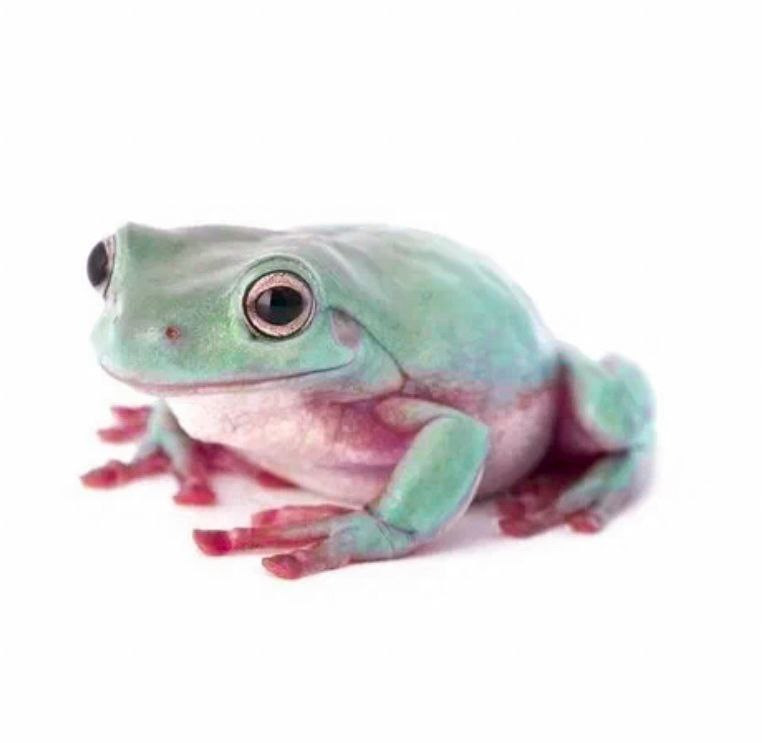
\includegraphics[width=0.4\textwidth]{https://raw.githubusercontent.com/vadyukkha/design_document_unity_game/refs/heads/main/pictures/photo_2024-12-01_22-21-33.jpg} 
    \caption{\textit {Референс главного персонажа}}
    \label{fig:example}
\end{wrapfigure} 
Аватар игрока (лягушка) представляет собой частично реалистичную лягушку. Окрас лягушки соответствует виду коралловопалая литория (рис. 1).  Лягушка передвигается прыжками, в  момент прыжка персонаж повёрнут в профиль. Профильная сторона детально прорисована в соответствии с референсным изображением. Механика прыжка и высовывания языка соответствуют действительной механике упомянутых движений коралловопалой литории. Исключением из реалистичности образа персонажа является механика передвижения под водой, высота и длина прыжка, вариация длины языка в большую сторону и наличие эмоций на морде. Соответствующие эмоции (радость, грусть) проявляются при успешном или неудачном прохождении уровня.

\subsection{Физическая модель}
Описание физической модели игрового мира, ее законов и их отображения в игру. 

\subsubsection{Перемещения}
Движение персонажа подчиняется классическим законам механики: 
\begin{itemize}
    \item Перемещение происходит по двум осям (X, Y) в системе координат игрового мира.
    \item Лягушка может прыгать, бегать и плавать под водой. Параметры, такие как высота и длина прыжка, зависят от скорости и продолжительности нажатия кнопки прыжка.
    \item Эффект гравитации воздействует на персонажа, что создает реалистичное ускорение вниз. Используется формула $a = g$, где $g = 9.8 \frac{м}{с^2}$, с возможными вариациями для уникальных миров.
\end{itemize}

\subsubsection{Боевые действия}
Боевая система включает следующие элементы:
\begin{itemize}
    \item Лягушка Лили атакует языком, выстреливая его в направлении цели. Дальность и скорость языка определяются формулой $v = v_0 + a \cdot t$, где $v_0$ — начальная скорость, $a$ — ускорение.
    \item Враги имеют уникальные зоны уязвимости и атакуют игрока по заданным паттернам.
    \item Урон врагу рассчитывается по формуле $D = P \cdot F_{crit}$, где $P$ — базовый урон, а $F_{crit}$ — множитель критического удара.
\end{itemize}

\subsubsection{Другие важные моменты}
\begin{itemize}
    \item \textbf{Столкновения:} Логика столкновений использует прямоугольные или круговые хитбоксы для определения взаимодействия между объектами.
    \item \textbf{Повреждения:} Игрок получает урон, если хитбокс врага касается Лили. Также возможна симуляция рикошета при столкновении с твердыми поверхностями.
    \item \textbf{Сопротивление среды:} В некоторых уровнях (например, под водой) на движения Лили влияет сопротивление, моделируемое по формуле $F = -k \cdot v$, где $k$ — коэффициент сопротивления, $v$ — скорость.
    \item \textbf{Моделирование разрушений:} Некоторые элементы игрового окружения могут разрушаться под воздействием игрока или врагов, например, ветки, которые ломаются под весом персонажа.
\end{itemize}

\end{document}
